\begin{frame}\frametitle{EURECOM Cloud Computing Platform}
\begin{itemize}
	\item {\bf Private datacenter, hosted at Eurecom}
	\begin{itemize}
		\item Few hundres of server slots
		\item Pretty immutable network configuration
		\item No service level agreements
	\end{itemize}

	\item {\bf Cloud Computing Platform}
	\begin{itemize}
		\item Hybrid system: VM-based and container-based
		\item $O(1000)$ cores, $O(2 TB)$ RAM, $O(200 TB)$ storage
		\item No service level agreements
	\end{itemize}
\end{itemize}
\end{frame}

\begin{frame}\frametitle{Zoe Analytics}
\begin{itemize}
	\item {\bf Towards datacenter operating systems}
	\begin{itemize}
		\item Cluster scheduler, in the family of Borg, Mesos, and K8s
		\item Geared toward Analytics applications
		\item Scheduler and Resource allocator
		\item Based on Docker containers
	\end{itemize}

	\item {\bf Eurecom Open Source project}
	\begin{itemize}
		\item You can contribute!
		\item A lot of interest from many companies
		\item A platform for research
	\end{itemize}
\end{itemize}
\end{frame}

\begin{frame}\frametitle{Jupyter Notebooks}

	\begin{figure}
		
\includegraphics[width=0.45\linewidth]{figures/jupyter}
	\end{figure}

	\begin{colorblock}{blue}{lightblue}{ }
   The Jupyter Notebook is a web application that allows you to create and share documents that contain live code, equations, visualizations and explanatory text. Uses include: data cleaning and transformation, numerical simulation, statistical modeling, machine learning and much more.
   \end{colorblock}
\end{frame}

\begin{frame}\frametitle{Zoe Jupyter Applications}
	\begin{figure}
		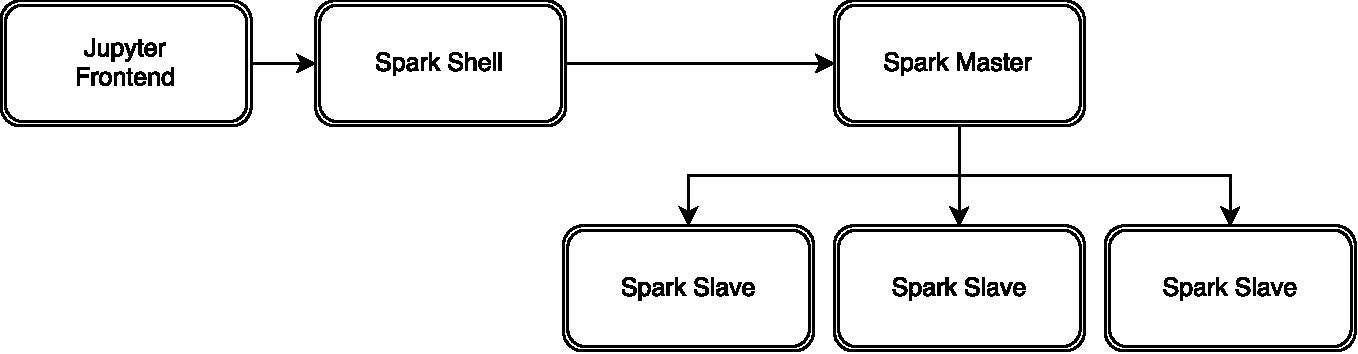
\includegraphics[scale=0.5]{figures/jupyter_app}
	\end{figure}
\end{frame}

\begin{frame}\frametitle{Working in the Lab}
\begin{itemize}
	\item {\bf Clone or Fork the AML-course repository}
	\item {\bf Working on your Notebook project}
	\begin{itemize}
		\item Upload your Notebook to the Zoe Jupyter application
		\item Work on your Notebook
		\item Download your Notebook as an iPython notebook
		\begin{itemize}
			\item This allows you to continue to work on your project during subsequent laboratory sessions, or eventually to work from home on a local installation
			\item It is strongly suggested to use GitHub!!
		\end{itemize}
	\end{itemize}
	\item {\bf Submitting your Notebook for evaluation}
	\begin{itemize}
		\item Download your Notebook as an html page
		\begin{itemize}
			\item Be careful! You need to save after you execute all cells!
		\end{itemize}
		\item Send by email the html version of the Notebook
	\end{itemize}
\end{itemize}
\end{frame}
